%! Author = Kevin Lin
%! Date = 11/3/2026

% Preamble
\documentclass[11pt,a4paper,margin=1in]{article}

% Packages
\usepackage{amsmath}
\usepackage{amssymb}
\usepackage{enumerate}
\usepackage{pdfpages}

\title{HW 6}
\author{Kevin Lin}
\date{11/3/2026}

% Document
\begin{document}
\maketitle

\section{}
\begin{enumerate}[(a)]
    \item Let $D^2 = \min_{2 \leq i \leq n}\|X_1 - X_i\|^2$. For $0 \leq t \leq 1$,
    define a disk $B(x, \sqrt{t}) = \{y : \|y - x\|_2 \leq \sqrt{t}\}$. Then, even
    in the worse case, when $x$ is at the corner of the unit square, at least
    one quarter of the disk lies inside the unit square. Therefore, $\text{Area}(B(x, \sqrt{t}) \cap [0, 1]^2) \geq \frac{1}{4}\pi(\sqrt{t})^2  = \frac{\pi t}{4}$. 
    Since $X_2, \cdots, X_n$ are independent and uniformly distributed in $[0, 1]^2$, 
    we have:
    \begin{align*}
        P(D^2 > t) &= P(X_i \notin B(x, \sqrt{t}) \text{ for all } i = 2, \cdots, n | X_1 = x) \\
        &= [1 - \text{Area}(B(x, \sqrt{t}) \cap [0, 1]^2)]^{n - 1} \\
        &\leq \left(1 - \frac{\pi t}{4}\right)^{n - 1}
    \end{align*}
    Use the fact that $1 - x \leq e^{-x}$ for all $x \in \mathbb{R}$, we have
    $P(D^2 > t | X_1 = x) \leq e^{-(n - 1)\pi t/4}$. This bound doesn't actually
    depend on $x$, so $P(D^2 > t) \leq e^{-(n - 1)\pi t/4}$ for $0 \leq t \leq 1$.
    Using the tail integral identity for a nonnegative random variable $X$, we have
    $E[D^2] = \int_0^\infty P(D^2 > t) dt$. Since any two points in the unit square
    are at most $\sqrt{2}$ apart, $D^2 \leq 2$, so we can bound the integral as follows:
    $E[D^2] = \int_0^1 P(D^2 > t) dt + \int_1^2 P(D^2 > t) dt$. 
    We can simplify the first term:
    \begin{align*}
        \int_0^1 P(D^2 > t) dt &\leq \int_0^1 e^{-(n - 1)\pi t/4} dt \\
        &\leq \int_0^\infty e^{-(n - 1)\pi t/4} dt \\
        &= \frac{4}{(n - 1)\pi}
    \end{align*}
    For $1 \leq t \leq 2$, $P(D^2 > t) \leq P(D^2 > 1) \leq e^{-(n - 1)\pi/4}$, 
    so we can bound the second term simply at $e^{-(n - 1)\pi/4}$. Therefore, we have
    $E[D^2] \leq \frac{4}{(n - 1)\pi} + e^{-(n - 1)\pi/4}$, which is $O(1/n)$,
    since for $n \geq 2$, $\frac{1}{n - 1} \leq \frac{2}{n}$ and exponential decay 
    is faster than $1/n$. Thus, there exists some absolute constant $C > 0$ such 
    that $E[D^2] \leq C/n$ for $n \geq 2$.
    \item Let $Z = f(X_1, \cdots, X_n)$, the total length of the shortest traveling
    salesman path through all $n$ points. We use the Efron-Stein inequality
    $Var(Z) \leq \sum_{i = 1}^{n}EVar^{(i)}(Z)$. For each $i$, let $Z_{-i} = f(X_1, \ldots, X_{i - 1}, X_{i + 1}, \\ \ldots, X_n)$, 
    the optimal path length after deleting $X_i$. Define the nearest neighbor distance
    of $X_i$ among the other points as $d_i = \min_{j \neq i}\|X_i - X_j\|_2$.
    We first show that $0 \leq Z - Z_{-i} \leq 2d_i$. The lower bound is trivial, 
    since removing a point cannot increase the optimal path length. For the upper
    bound, let $X_j$ be the nearest neighbor of $X_i$ so that their distance
    is $d_i$. Start with an optimal path through $n - 1$ points excluding $X_i$, 
    then insert $X_i$ between $X_j$ and $X_k$, its nearest neighbor. The increase
    in path length is consequently $\|X_j - X_i\|_2 + \|X_i - X_k\|_2 - \|X_j - X_k\|_2$.
    By the triangle inequality, $\|X_j - X_k\|_2 \leq \|X_j - X_i\|_2 + \|X_i - X_k\|_2$,
    so the increase in path length is at most $2\|X_j - X_i\|_2 = 2d_i$. Therefore, 
    $0 \leq Z - Z_{-i} \leq 2d_i$.

    For fixed $X_{-i}, Z_{-i}$ is constant with respect to $X_i$. For any 
    random variable $Y$ and constant $a$, $Var(Y) = E[(Y - a)^2] - (E[Y] - a)^2 \leq E[(Y - a)^2]$. 
    since the mean minimizes the mean squared error. Therefore, conditionally on
    $X_{-i}$, we have $Var^{(i)}(Z) \leq E^{(i)}[(Z - Z_{-i})^2] \leq E^{(i)}[4d_i^2] = 4E^{(i)}[d_i^2]$. 
    Taking the expectation over the remaining variables, we have $EVar^{(i)}(Z) \leq 4E[d_i^2]$. 
    By Efron-Stein, $Var(Z) \leq \sum_{i = 1}^{n}EVar^{(i)}(Z) \leq 4\sum_{i = 1}^{n}E[d_i^2]$.
    Since all $X_i$ are iid, all $d_i$ follow the same distribution, so $Var(Z) \leq 4nE[d_1^2]$. 
    By part (a), $Var(Z) \leq 4nE[d_1^2] = O(1)$, since $E[d_1^2] = O(1/n)$, thus
    $Var(Z) \leq C$ for some absolute constant $C > 0$.
\end{enumerate}

\section{}
Let $X \sim \text{Exp}(1)$ and $g : \mathbb{R} \to \mathbb{R}$ be bounded with
a bounded derivative. Define $h(x) = g(x) - g(0)$, so that $h(0) = 0$ and $h'(x) = g'(x)$.
Since variance is unchanged by subtracting a constant, $Var(g(X)) = Var(h(X))$,
then $Var(h(X)) = E[h(X)^2] - (E[h(X)])^2 \leq E[h(X)^2]$. Now, using the hint
and since $(h(x)^2)' = 2h(x)h'(x)$, we have:
\begin{align*}
    E[h(X)^2] &= \int_0^\infty h(x)^2 e^{-x} dx \\
    &= h(0)^2 + \int_0^\infty 2h(x)h'(x) e^{-x} dx \\
    &= 2E[h(X)h'(X)]
\end{align*}
Then, by Cauchy-Schwarz
\begin{align*}
    E[h(X)h'(X)] &\leq 2\sqrt{E[h(X)^2]E[h'(X)^2]} \\
    \sqrt{E[h(X)^2]} &\leq 2\sqrt{E[h'(X)^2]} \\
    E[h(X)^2] &\leq 4E[h'(X)^2] \\
    Var(g(X)) &= Var(h(X)) \\ 
    &\leq E[h(X)^2] \\
    &\leq 4E[h'(X)^2] \\
    &= 4E[g'(X)^2]
\end{align*}
Thus, the one dimensional Poincare inequality is $Var(g(X)) \leq 4E[g'(X)^2]$.
Now, we expand to $n$ dimensions using the Efron-Stine inequality. Let $Z = f(X_1, \ldots, X_n)$. 
Fix $i \in \{1, \ldots, n\}$ and let $g_i(x) = f(X_1, \ldots, X_{i - 1}, x, X_{i + 1}, \ldots, X_n)$. Because
$f$ and its first partial derivatives are bounded, $g_i$ is bounded with a bounded derivative.
$g_i'(x) = \frac{\partial f}{\partial x_i}(X_1, \ldots, X_{i - 1}, x, X_{i + 1}, \ldots, X_n)$.
Since $X_i$ is independent of $X_{-i}$, its conditional distribution given $X_{-i}$
remains $\text{Exp}(1)$. Therefore, we can apply the one dimensional Poincare inequality:
\begin{align*}
    Var^{(i)}(f(X_1, \ldots, X_n)) &= Var(g_i(X_i) | X_{-i}) \\
    &\leq 4E[g_i'(X_i)^2 | X_{-i}] \\
    &= 4E\left[\left(\frac{\partial f}{\partial x_i}(X_1, \ldots, X_n)\right)^2 | X_{-i}\right] \\
    E[Var^{(i)}(Z)] &\leq 4E\left[E\left[\left(\frac{\partial f}{\partial x_i}(X_1, \ldots, X_n)\right)^2 | X_{-i}\right]\right] \\
    &= 4E\left[\left(\frac{\partial f}{\partial x_i}(X)\right)^2\right]
\end{align*}
Now, use Efron-Stein:
\begin{align*}
    Var(f(X)) &\leq \sum_{i = 1}^{n}E[Var^{(i)}(Z)] \\
    &\leq 4\sum_{i = 1}^{n}E\left[\left(\frac{\partial f}{\partial x_i}(X)\right)^2\right] \\
    &= 4E\left[\sum_{i = 1}^{n}\left(\frac{\partial f}{\partial x_i}(X)\right)^2\right]
\end{align*}
By the definition of the squared Euclidean norm of the gradient, $\|\nabla f(X)\|_2^2 = \sum_{i = 1}^{n}\left(\frac{\partial f}{\partial x_i}(X)\right)^2$, 
thus $Var f(X_1, \ldots, X_n) \leq 4E[\|\nabla f(X_1, \ldots, X_n)\|_2^2]$, which 
is the $n$-dimensional Poincare inequality.

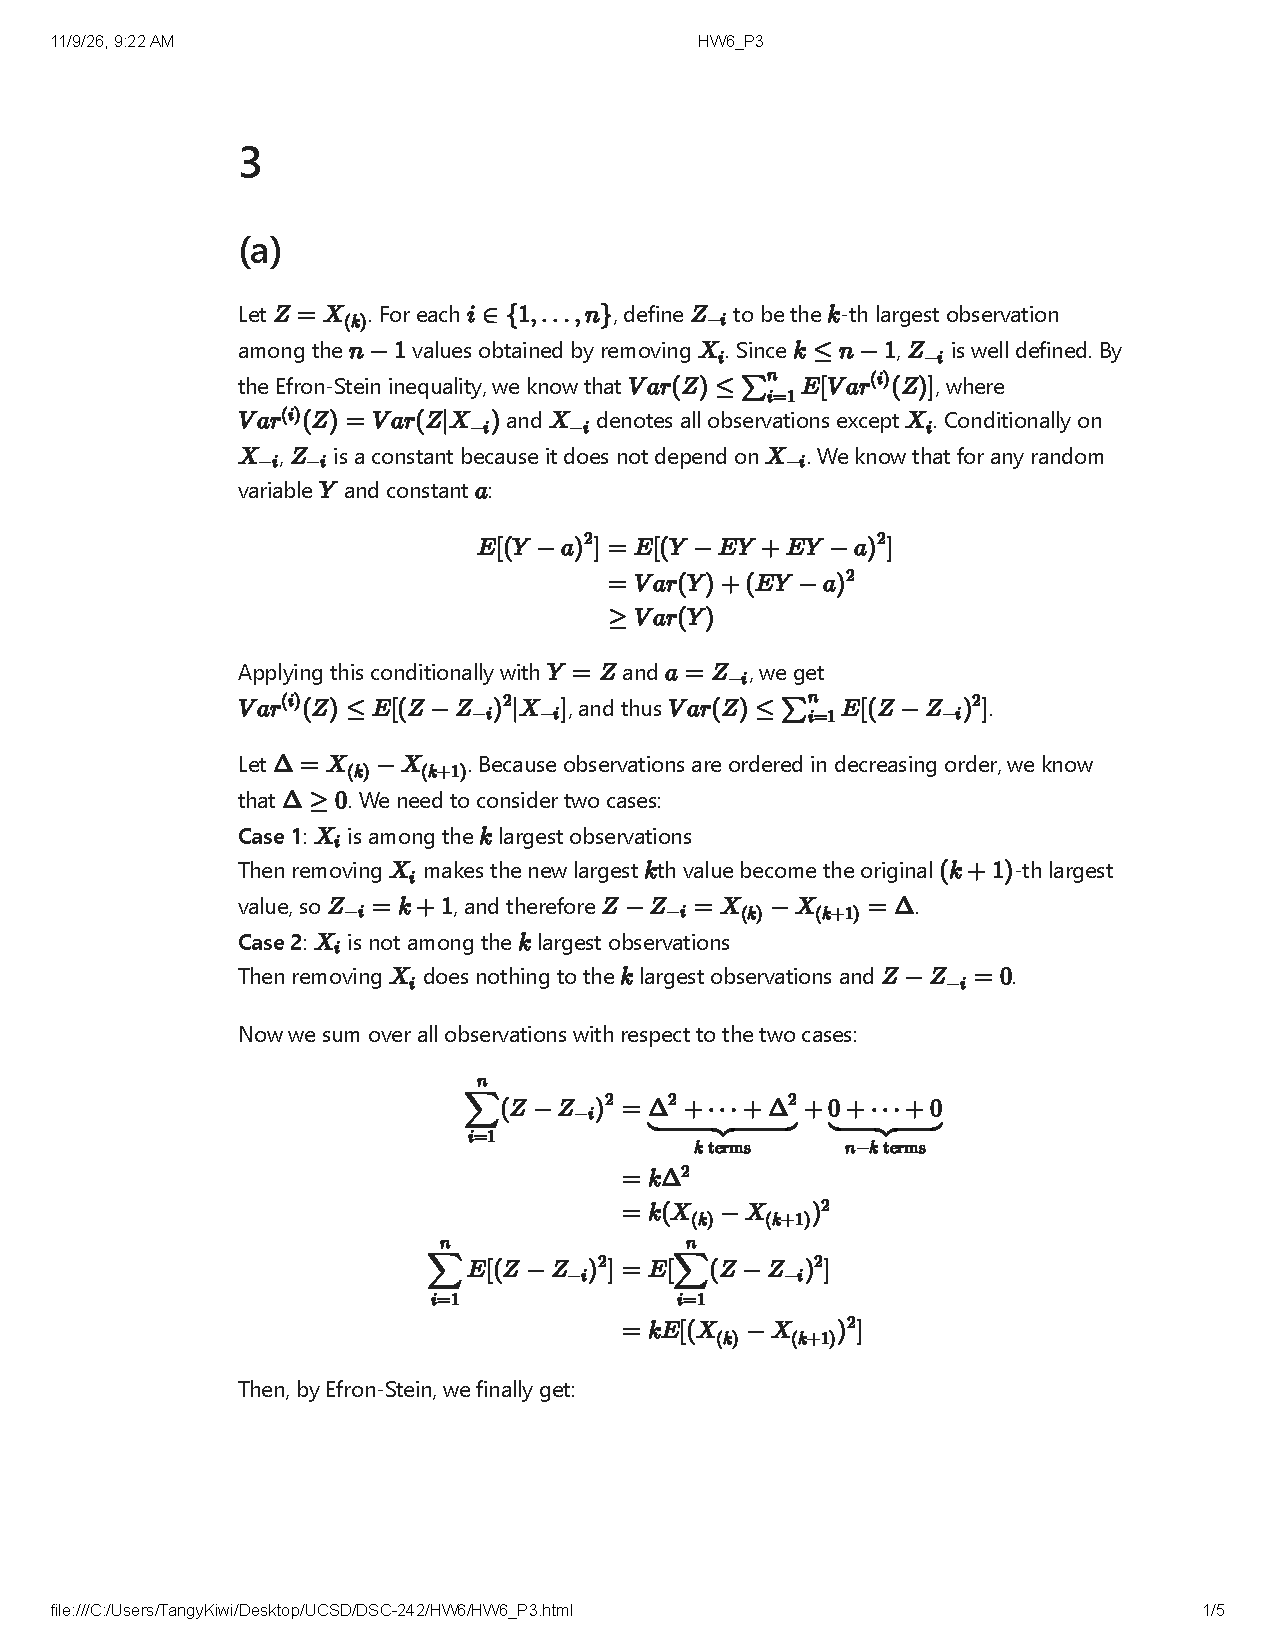
\includepdf[pages=-]{HW6_P3.pdf}

\section{}
Let $Z = X - EX$, then $EZ = 0$, and since $Z$ is $\frac{\sigma^2}{4}$-subgaussian,
we have $E[e^{\lambda Z}] \leq e^{\frac{\lambda^2\sigma^2}{8}}$ for all $\lambda \in \mathbb{R}$.
Define the log MGF as $\psi(\lambda) = \log E[e^{\lambda Z}]$. Then, $\psi(0) = 0$
and $\psi(\lambda) \leq \frac{\lambda^2\sigma^2}{8}$. Now use Jensen's inequality
to get that $E[e^{\lambda Z}] \geq e^{\lambda EZ} = 1$, so $\psi(\lambda) \geq 0$.
Combining these inequalities gives us $0 \leq \psi(\lambda) \leq \frac{\lambda^2\sigma^2}{8}$ 
for all $\lambda \in \mathbb{R}$, which also guarantees that the MGF is finite
for every real $\lambda$ and $\psi$ is differentiable. \\

\noindent
Since $\log(e^{\lambda Z}) = \lambda Z$, we can use the provided entropy function
to get $\text{Ent}(e^{\lambda Z}) = \lambda E[Ze^{\lambda Z}] - E[e^{\lambda Z}]\log E[e^{\lambda Z}]$.
Now, from $\psi$, we know $E[e^{\lambda Z}] = e^{\psi(\lambda)}$ and $E[Ze^{\lambda Z}] = \psi'(\lambda)e^{\psi(\lambda)}$, 
so we can rewrite the entropy as $\text{Ent}(e^{\lambda Z}) = \lambda \psi'(\lambda)e^{\psi(\lambda)} - e^{\psi(\lambda)}\psi(\lambda) = E[e^{\lambda Z}](\lambda \psi'(\lambda) - \psi(\lambda))$.
Thus, it suffices to prove that $\lambda \psi'(\lambda) - \psi(\lambda) \leq \frac{\lambda^2\sigma^2}{8}$ 
for all $\lambda \in \mathbb{R}$. \\

\noindent
Define the exponentially tilted probability distribution $\frac{dP_\lambda}{dP} = \frac{e^{\lambda Z}}{E[e^{\lambda Z}]}$.
Differentiating twice gives us $\psi''(\lambda) = \frac{E[Z^2e^{\lambda Z}]}{E[e^{\lambda Z}]} - \left(\frac{E[Ze^{\lambda Z}]}{E[e^{\lambda Z}]}\right)^2 = E_\lambda[Z^2] - (E_\lambda[Z])^2 = Var_\lambda(Z)$, 
where $E_\lambda$ and $Var_\lambda$ are the expectation and variance under the 
tilted distribution $P_\lambda$, which ultimately $Var_\lambda(Z) \geq 0$, and thus
the log MFG is convex. For any differentiable convex function, $\psi(b) \geq \psi(a) + \psi'(a)(b - a)$.
Choose $a = \lambda$, $b = 2\lambda$, then $\psi(2\lambda) \geq \psi(\lambda) + \psi'(\lambda)\lambda$, 
which we can simplify:
\begin{align*}
    \psi(2\lambda) &\geq \psi(\lambda) + \psi'(\lambda)\lambda \\
    \lambda\psi'(\lambda) &\leq \psi(2\lambda) - \psi(\lambda) \\
    \lambda\psi'(\lambda) - \psi(\lambda) &\leq \psi(2\lambda) - 2\psi(\lambda) \leq \psi(2\lambda) \\
    \lambda\psi'(\lambda) - \psi(\lambda) &\leq \frac{(2\lambda)^2\sigma^2}{8} = \frac{\lambda^2\sigma^2}{2}
\end{align*}
Now apply this to the entropy function to get $\text{Ent}(e^{\lambda Z}) \leq \frac{\lambda^2\sigma^2}{2}E[e^{\lambda Z}]$.
Recall since $X = Z + EX$, we have $e^{\lambda X} = e^{\lambda EX}e^{\lambda Z}$.
For any positive constant $c$ and positive random variable $Y$:
\begin{align*}
    \text{Ent}(cY) &= E[cY\log(cY)] - E[cY]\log E[cY] \\
    &= cE[Y\log(cY)] - cE[Y]\log(cE[Y]) \\
    &= cE[Y(\log c + \log Y)] - cE[Y](\log c + \log E[Y]) \\
    &= cE[Y\log Y] + cE[Y]\log c - cE[Y]\log E[Y] - cE[Y]\log c \\
    &= c(E[Y\log Y] - E[Y]\log E[Y]) \\
    &= c\text{Ent}(Y)
\end{align*}
Now apply this with $c = e^{\lambda EX}$:
\begin{align*}
    \text{Ent}(e^{\lambda X}) &= \text{Ent}(e^{\lambda EX}e^{\lambda Z}) \\
    &= e^{\lambda EX}\text{Ent}(e^{\lambda Z}) \\
    &\leq e^{\lambda EX}\frac{\lambda^2\sigma^2}{2}E[e^{\lambda Z}] \\
    &= \frac{\lambda^2\sigma^2}{2}E[e^{\lambda EX}e^{\lambda Z}] \\
    &= \frac{\lambda^2\sigma^2}{2}E[e^{\lambda X}]
\end{align*}
Thus, $\text{Ent}(e^{\lambda X}) \leq \frac{\lambda^2\sigma^2}{2}E[e^{\lambda X}]$ 
for all $\lambda \in \mathbb{R}$.

\noindent 
\textbf{AI Usage:} All homework problems were written in VSCode and compiled using LaTeX
(Problem 3 utilized Jupyter notebook), with assistance from ChatGPT and Github 
Copilot inline suggestions.


\end{document}